% !!!!!!!!!!!!!!!!!!!!!!!!!!!!!!!!!!!!!!!!!!!!!!!!!!!!!!!!!!!!!!!!!!!!!!!!!!!!
%                                                                            !
% Adapt this file so that you can use it for your thesis					 !
%                                                                            !
% !!!!!!!!!!!!!!!!!!!!!!!!!!!!!!!!!!!!!!!!!!!!!!!!!!!!!!!!!!!!!!!!!!!!!!!!!!!!


\documentclass{micro-econ-thesis}
\usepackage{graphicx}
\usepackage{setspace}
\usepackage{float}
\usepackage[utf8]{inputenc} % depends on the font encoding that you are using

% For formatting of your bibliography, please use the following package with options 
\usepackage[style=authoryear]{biblatex}
\usepackage{gensymb}
\usepackage{amsmath}
\usepackage{booktabs}

\usepackage{chngcntr}
\counterwithout{table}{section}

\addbibresource{bibliography.bib} % add a bib-reference file

\begin{document}
% ----------------------------------------------------------------------------
% Details for the titlepage
% ----------------------------------------------------------------------------
\thesisTitle{Development of Analysis Techniques for dynamic magnetic resonance imaging}
\thesisType{Master Thesis} % 'Master Thesis' or 'Seminar Paper'
\thesisAuthor{Aayush Nepal}
\thesisMail{aayush.nepal@uni-jena.de}
\thesisGrade{Master of Science in Medical Photonics} % leave empty for seminar papers
\thesisTutora{Prof. Dr. rer. nat. med. habil. Jürgen Reichenbach}
\thesisTutorb{Dr. rer. nat. Martin Krämer}
\thesisMatrikel{198683}
\thesisAddress{Schützenggase 2\\[.5ex]
								99423 Weimar}
\thesisDate{\today}
% In case of external supervisor
\thesisCompany{}

% Print titlepage
\thesisMakeTitle

% ----------------------------------------------------------------------------
% Abstract
% ----------------------------------------------------------------------------
\cleardoublepage
\pagenumbering{roman}
\pagestyle{plain}
%\thispagestyle{empty}
\subsection*{Abstract}


\clearpage
\subsection*{Acknowledgements}


% ----------------------------------------------------------------------------
% Table of contents
% ----------------------------------------------------------------------------
\cleardoublepage
%\thispagestyle{empty}
\tableofcontents

% ----------------------------------------------------------------------------
% List of figures/tables
% ----------------------------------------------------------------------------
\cleardoublepage
\phantomsection
\addcontentsline{toc}{section}{List of Figures}
\listoffigures
% --------------------------
\cleardoublepage
\phantomsection
\addcontentsline{toc}{section}{List of Tables}
\listoftables
% --------------------------

\cleardoublepage
\phantomsection
\addcontentsline{toc}{section}{List of Acronyms}
\section*{List of Acronyms}
\begin{tabular}{@{}ll}
FSU Jena & Friedrich-Schiller-Universität Jena\\
\end{tabular}

% --------------------------

% ----------------------------------------------------------------------------
% Contents
% ----------------------------------------------------------------------------
\cleardoublepage
\pagestyle{headings}
\pagenumbering{arabic}
\setcounter{page}{1}
% Contents
\onehalfspacing % for linespacing 1.5, you can turn it off with \singlespacing, e.g. for quotes or tables with multiline cells


\section{Introduction}
\label{sec:intro}


\subsection{The Knee Joint }
The knee joint, a pivotal structure in the human body, plays an essential role in locomotion. Additionally, it functions to control the center of body mass and posture in the activities of daily living by facilitating a wide range of movements. As such, the knee's health and integrity are vital for overall quality of life, influencing everything from basic mobility to participation in complex sports. A comprehensive survey across 15 European countries and Israel found that knee pain was the third most commonly reported type of chronic pain. This underscores the significant public health concern it represents \parencite{breivik_survey_2006}. Furthermore, arthritis/osteoarthritis (OA) was identified as the most common cause of this pain. 

This situation has not improved over time. In Germany for instance, a recent retrospective study has found that the number of patients with OA is steadily rising \parencite{obermuller_epidemiology_2024}. 
Knee-related issues are prevalent and impactful due to the inherent complexity of the knee joint itself. As a hub of various anatomical structures working in unison, the knee supports a range of movements and bears significant loads, making it susceptible to a variety of injuries and conditions.
Understanding the anatomy of the knee is the first step in tackling this problem. 

\textbf{Anatomy and Function}

The knee joint is the largest and the most superficial synovial joint in the body. \parencite{dalley_moores_2023}. 
It comprises three primary articulations:two femorotibial articulations (see Figure \ref{fig:rightkneeplate519}) and one femoropatellar articulation. These articulations, illustrated in figures \ref{fig:rightkneeplate519} and \ref{fig:patellarsurface}, are defined by their complexity and incongruence, features that are crucial for the joint's biomechanical performance. 
 
\begin{figure}[H]
	\centering
	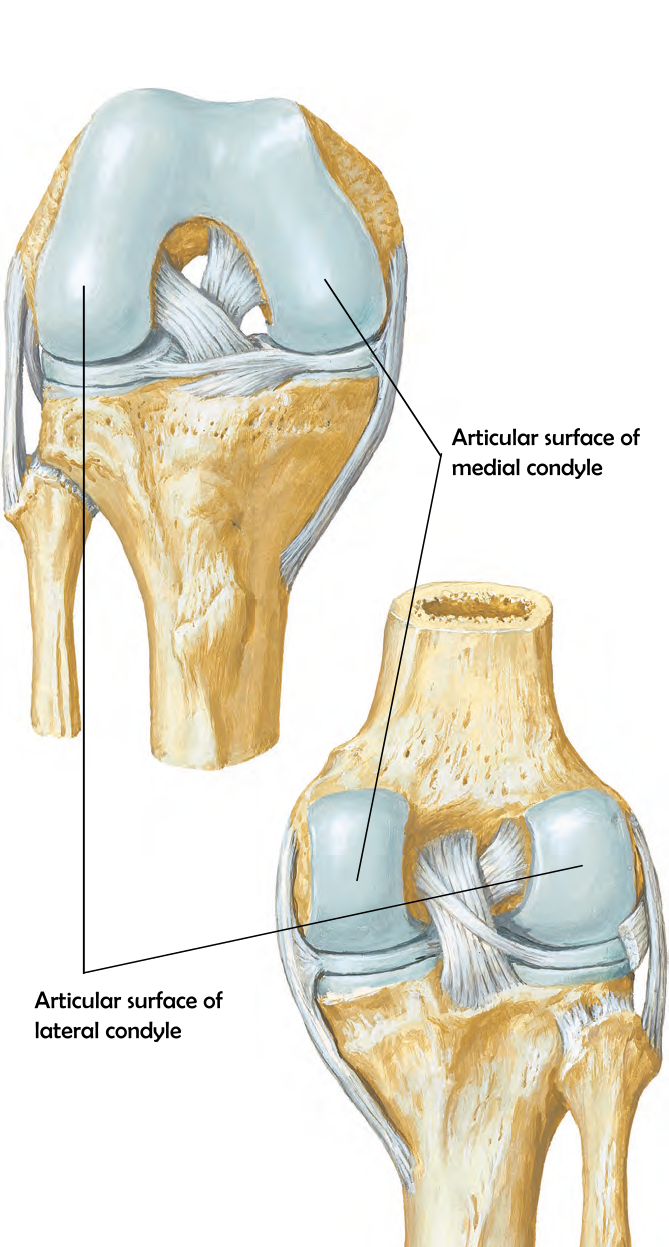
\includegraphics[width=0.7\linewidth]{right_knee_labeled}
	\caption{Anterior (flexed,top) and posterior (extended, bottom) view of the right knee with their articular surfaces labeled. \parencite[p.519]{netter_519_2023}}
	\label{fig:rightkneeplate519}
\end{figure}

\begin{figure} [H]
	\centering
	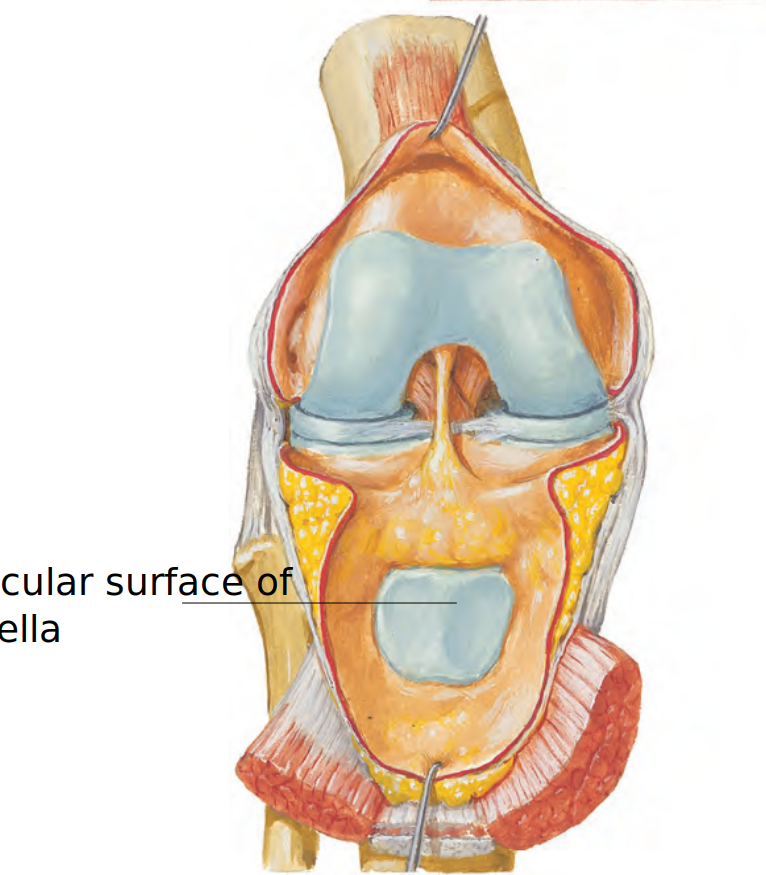
\includegraphics[width=0.7\linewidth]{patellar_surface}
	\caption[patellar surface]{Right joint opened, knee slightly in flexion, with the patellar articulation labelled. \parencite[p.517]{netter_519_2023}}
	\label{fig:patellarsurface}
\end{figure}

This design allows the knee to manage a wide array of movements and bear significant loads. Figure \ref{fig:sixdegrees} illustrates the knee's capacity for multidimensional movement, highlighting the joint's sophisticated structural design that enables this versatility. However, this inherent design also renders the knee vulnerable to a range of forces \parencite{standring_grays_2021}.

Such mechanical forces, influenced by activities and body mass index (BMI), are significant causes of OA and represent one of the most modifiable risk factors \parencite{heidari_knee_2011}. Furthermore, abnormal joint loading is considered a key mechanical driver of osteochondral changes thought to contribute to the initiation and progression of knee OA \parencite{coburn_immediate_2023}.

\begin{figure}[H]
	\centering
	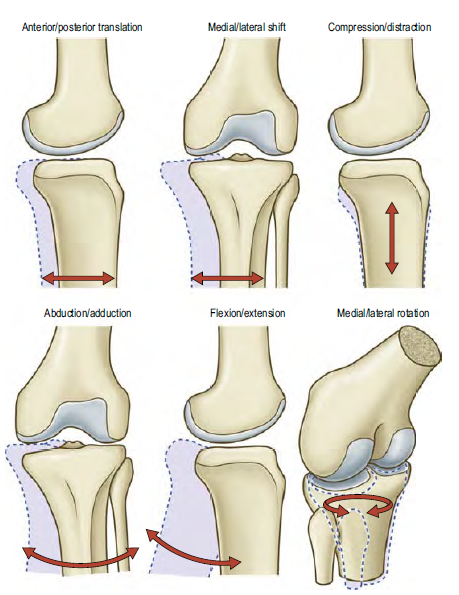
\includegraphics[width=0.7\linewidth]{six_degrees}
	\caption{The knee joint motion in three dimensions, described using six independent variables (degrees of freedom) \parencite[p.~1412]{standring_grays_2021}.}
	\label{fig:sixdegrees}
\end{figure}

The relationship between biomechanical stresses and knee health highlights the need for diagnostic tools that fulfill two key criteria: they must capture the knee's dynamic behavior during motion and assess the joint under varying loads. Dynamic magnetic resonance imaging (MRI) excels in meeting these requirements as one of the most advanced imaging modalities.

\subsection{Dynamic MRI}
In a broad sense, dynamic MRI is an umbrella term encompassing various MRI techniques designed to capture and visualize physiological processes and motion over time. The dynamic aspect of MRI is crucial for studying systems or structures involving inherent motion, such as blood flow, tissue perfusion, or cardiac activity. For the purposes of this project, the focus of "dynamic MRI" narrows down to capturing the bulk movement of the knee joint undergoing active flexion extension cycles inside the scanner. Compared to traditional static MRI scans, which are highly susceptible to motion artifacts compared to other imaging modalities \parencite{zaitsev_motion_2015}, dynamic MRI techniques not only accommodates motion, but can even leverage it to offer comprehensive insights into the functional and biomechanical properties of the concerned structures.  Among these techniques, CINE imaging, particularly renowned in cardiac MRI, is considered the gold standard for evaluating cardiac function \parencite{menchon-lara_reconstruction_2019}. Its high regard in cardiac MRI demonstrates the method's precision and adaptability—traits that are leveraged in knee imaging.

\subsubsection{CINE imaging}

CINE, derived from 'cinematography,' refers to creating a movie-like sequence of images. In the context of dynamic knee MRI, this technique can be used to reconstruct a "movie" of a single flexion-extension cylce. This visualization is achieved by aggregating multiple partial datasets acquired over various cycles. The knee's movement cycle is segmented into distinct stages, each corresponding to a specific angle of flexion or extension. For each stage, k-space — the Fourier transform space from which MR images are reconstructed — is incrementally sampled. This data is gathered across multiple repetitions of the movement cycle, ensuring comprehensive coverage of k-space and thus, high-resolution imaging of each movement phase.This technique works robustly only if the cycles are sufficiently similar \parencite{curtis_primer_2022}. Achieving this consistency in dynamic MRI of the knee, which naturally involves significant movement variations, requires precise synchronization of the imaging process.

\subsubsection{Gating} 

This synchronization, known as gating, aligns image acquisition with specific, repeatable points in the knee's movement cycle. By ensuring each captured image corresponds accurately to a consistent phase of motion, it minimizes the discrepancies that can arise from cycle-to-cycle variations, enhancing the reliability of bio-mechanical analyses. Although there are two types of gating, namely prospective and retrospective, it is the latter that is the standard for CINE imaging as it provides a more consistent image quality \parencite[p. 102]{edelman_clinical_1996}. In retrospective gating, the data is acquired continuously throughout the motion cycle. The data is then reordered post-acquisition into a coherent sequence that shows the knee at different positions along the motion cycle. This necessitates external information that captures the precise moment and position of the knee throughout its range of movement beyond just the raw data acquired during the MRI scan. A previously reported novel knee loading device is employed to address this, which comes with an optical sensor attachment that provides this vital information \parencite{brisson_novel_2022}. 

\subsubsection{Knee loading device }

The MR-compatible knee loading device employed in this study is illustrated in Figure \ref{fig:kneedevice}. This device allowed for a range of motion of approximately 25 to 45 degrees (subject-dependent), enabling subjects to perform knee flexion and extension cycles under both loaded and unloaded conditions. For loading, the device was equipped with compartments for weight plates and sandbags, providing a physiological load of 10 to 12 kilograms. These weights are positioned at the distal end of the device, directly influencing the mechanics of knee extension. As the subject extends the knee, they must overcome not only the natural resistance of their body weight but also the additional external load imposed by these weights. Central to this device's functionality is an optical fiber position sensor (MR338-Y10C10, Micronor, 155 Camarillo, CA, USA), which precisely  measures the ab­solute angle from 0{\degree}\,to 360\degree \, with a resolution of 0.025\degree \parencite{rickenbach_optical_2013}. This measurement capability is critical for synchronizing the knee's movement with MRI data reconstruction. 
\begin{figure} [H]
	\centering
	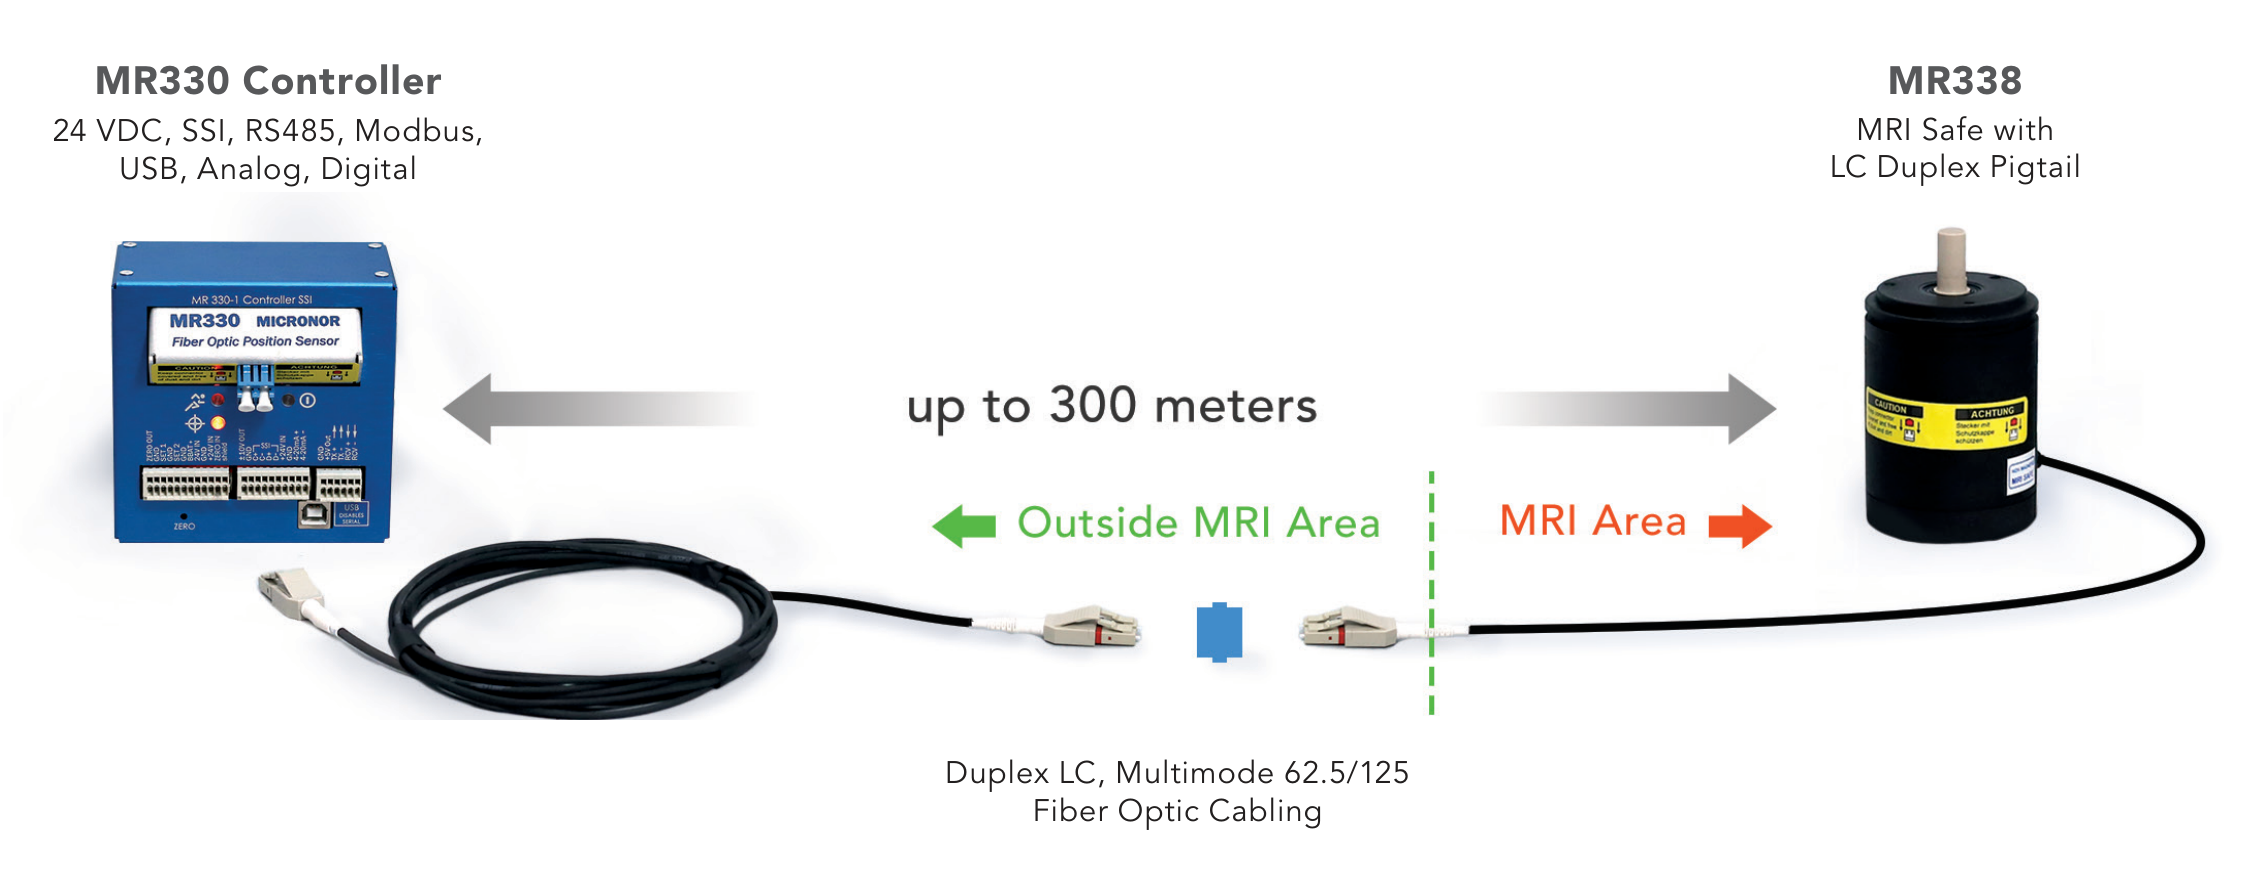
\includegraphics[width=0.7\linewidth]{sensor_img}
	\caption{The MR330 controller (left) and MR338 optical fiber position sensor system (right), showcasing the connection from the controller to the sensor via duplex LC multimode fiber optic cabling.}
	\label{fig:sensorimg}
\end{figure}


As shown in Figure \ref{fig:sensorimg} , the MR330 controller interfaces with the MRI-safe MR338 position sensor to facilitate precise measurement within the MRI environment, accommodating up to 300 meters of fiber optic cabling. The controller is connected to a laptop placed outside the scanner while the sensor is attached to the device within. To enhance signal acquisition and the clarity of imaging, two flexible coils \underline{(cite the coils here, perhaps also show a picture)} were positioned at key anatomical locations: one at the distal femur and another at the proximal tibia, as specified in the MRI protocol.
\begin{figure}[H]
	\centering
	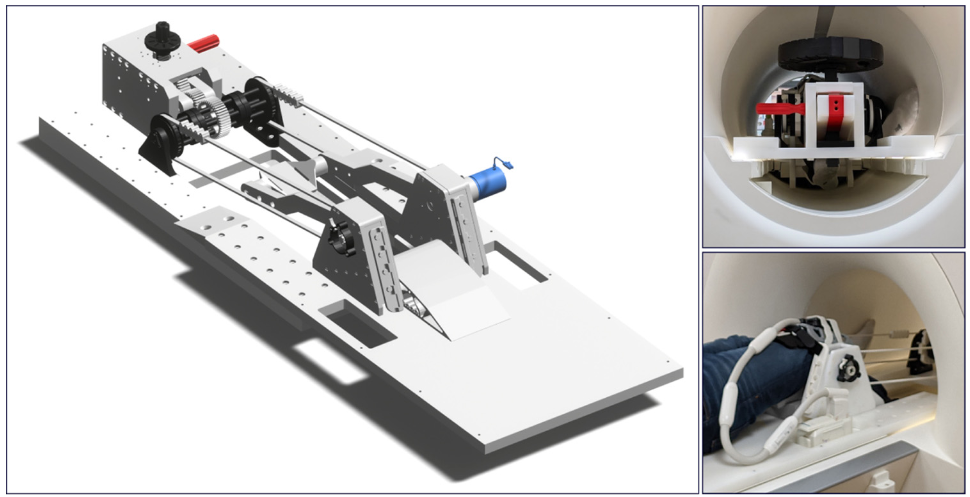
\includegraphics[width=0.9\linewidth]{knee_device}
	\caption{A 3D rendering of the knee motion/loading device (left) and two photographs of the device in a Siemens Magnetom Prisma Fit MRI scanner (right). The top right image (rear view) demonstrates how the distal part of the device sits atop the rails within the scanner bore, which are normally used to guide and support the patient table. The bottom right image (front, oblique view) demonstrates an individual positioned in the device with a flexible coil around the index knee, the thigh secured between the proximal pillow blocks and the ankle fastened to the leg support, as well as the coil plug setup.}
	\label{fig:kneedevice}
\end{figure}
 


  
To further enhance the quality and precision of our imaging, and to maximize the potential for precise image reconstruction, a previously reported radial golden-angle gradient-echo FLASH sequence was used, which is more robust against motion artifacts than Cartesian sequences \parencite{aleksiev_high-resolution_2022}. The following sections will detail the key components of this technique — radial golden-angle acquisition and the gradient-echo FLASH sequence.

\subsubsection{Radial golden-angle acquisition}


As the name suggests, radial golden-angle acquisition specifically modifies how k-space is sampled. Unlike traditional static MRI, which typically employs Cartesian sampling, this method utilizes radial sampling. Here, the data points are collected along radial lines spreading out from the center of k-space, resembling spokes on a wheel. Figure \ref{fig:radial} depicts a generic radial sampling scheme. The separation between any two adjacent circles defines the separation $\Delta k_r$ in the radial sampling direction, whereas, the angular separation between any two successive angular lines in k-space (such as between the two example lines shown in the figure) defines $\Delta \theta$. The two quantities $\Delta k_r$ and $\Delta \theta$ are constrained by the Nyquist sampling criterion. \parencite{brown_magnetic_2014} 
  
 \begin{figure}[H]
 	\centering
 	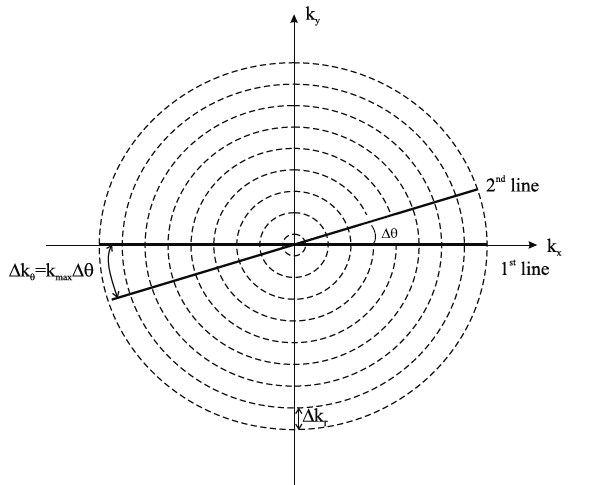
\includegraphics[width=0.7\linewidth]{radial}
 	\caption{Generic radial k-space sampling \parencite[p.306]{brown_magnetic_2014}}
 	\label{fig:radial}
 \end{figure}
 
 The 'golden-angle' strategy, which we employ, optimizes this approach by spacing the radial lines at an angle of approximately 111.25 degrees. This specific angle helps in evenly covering the k-space without overlapping, ensuring that each new image frame provides unique information, thus enhancing image quality and temporal resolution. 
 
\begin{figure}[H]
	\centering
	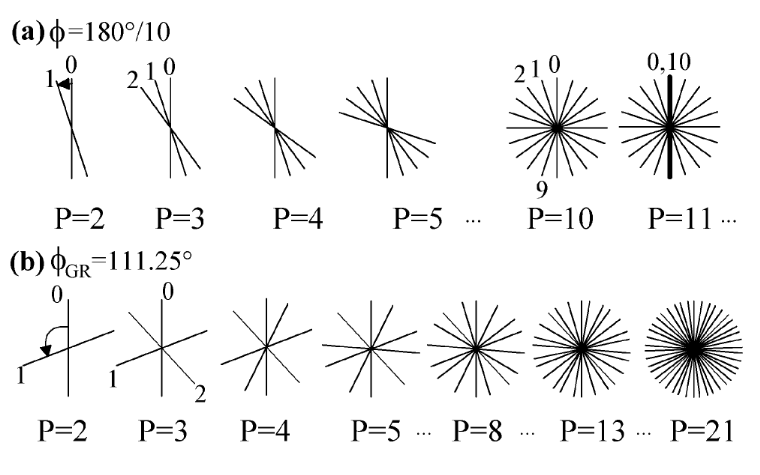
\includegraphics[width=0.7\linewidth]{golden_angle_figure}
	\caption{Radial k-space sampling strategies. (a) Fixed angular increment, showing potential for uneven k-space coverage. (b) Golden-angle sampling, ensuring uniform distribution across k-space \parencite{winkelmann_optimal_2007}.}
	\label{fig:goldenanglefigure}
\end{figure}

 
Figure \ref{fig:goldenanglefigure} provides a visual comparison between traditional fixed increment and the golden-angle methods in k-space sampling. It highlights how each approach affects the distribution of sampling lines across k-space. In the figure, part (a) shows radial sampling using a fixed angular increment. This traditional method can lead to gaps or overlaps in data collection, depending on the number of radial profiles used. Part (b) demonstrates the golden-angle method, where each new radial line is placed at an increment of approximately 111.25 degrees. This approach allows for a more uniform distribution of sampling lines across the k-space, enhancing image quality by preventing gaps and reducing redundancy in data collection. Figure blank  shows the k-space of a specific frame during the knee flexion cycle and the corresponding reconstructed MRI image.
\begin{figure}[H]
	\centering
	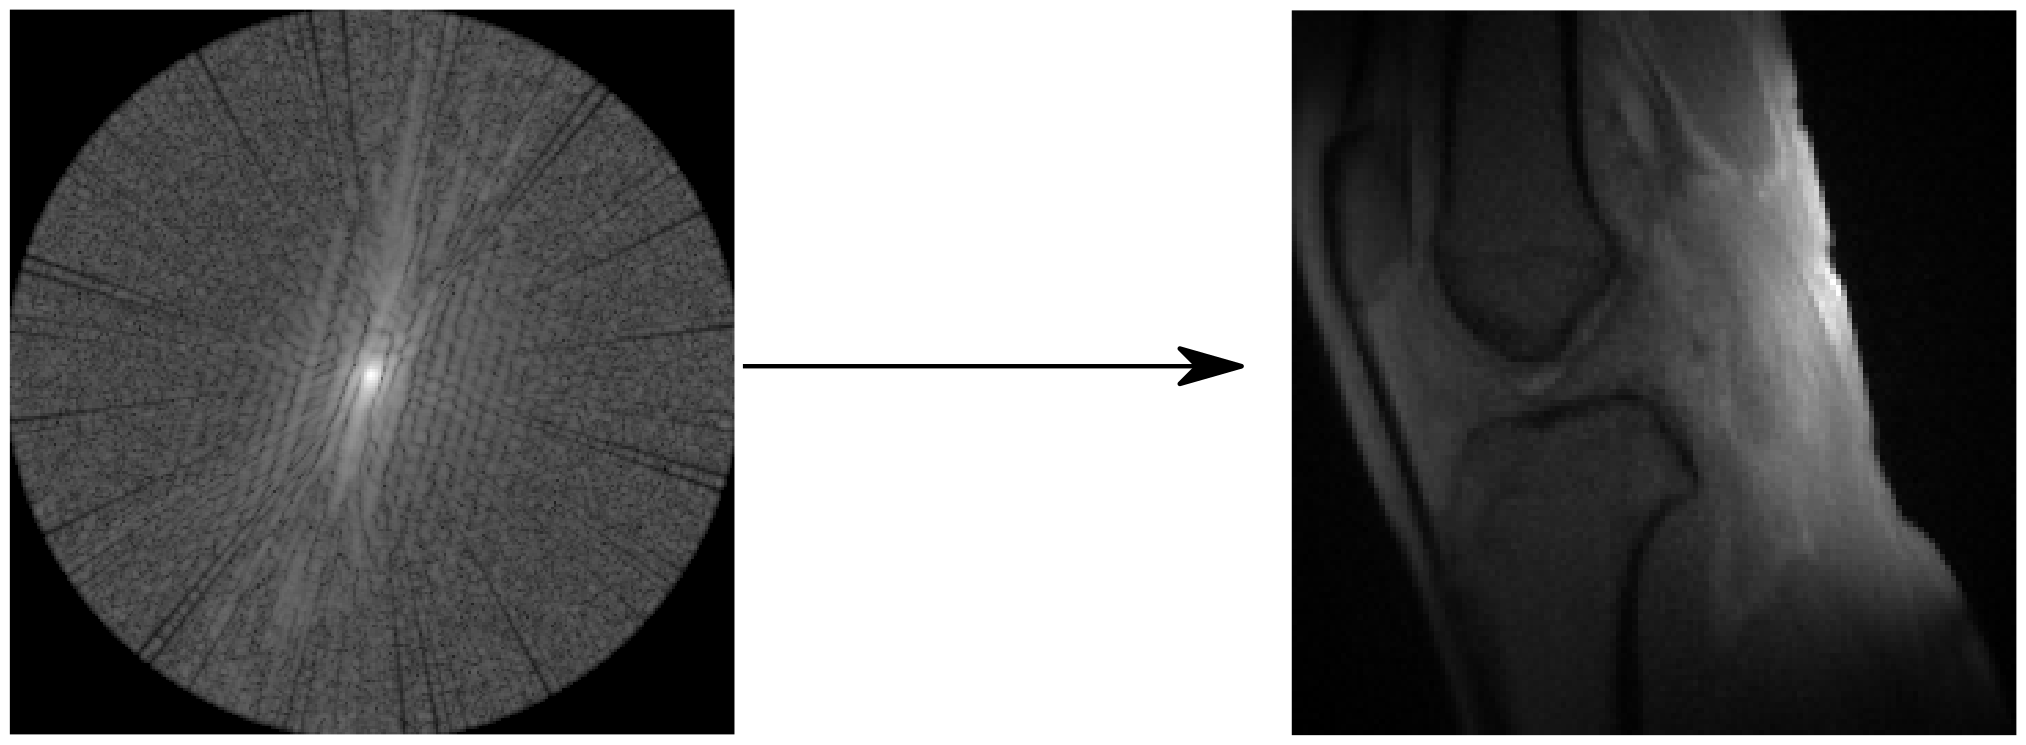
\includegraphics[width=0.9\linewidth, height=7.3cm]{kspace_arrow}
	\caption{\textbf{Example of k-space and reconstructed image}. Left: K-space data from a specific angle during the knee flexion cycle. Right: Corresponding reconstructed MRI image, illustrating the detailed visualization achievable through golden-angle sampling.}
	\label{fig:kspacearrow}
\end{figure}
  
\subsubsection{Gradient Echo FLASH sequence}

Gradient echo (GRE) is a prime candidate for dynamic MRI because it is a fast scanning process. There are two major factors that contribute to its speed. First, unlike the spin echo, we do not need to wait for a long time for the longitudinal magnetization component $M_z$ to sufficiently recover for another repetition. This is because in a GRE sequence, a smaller flip angle is used. Secondly, we do not need to wait for the spins to refocus after the application of a $180^o$ rf pulse, because there is no such pulse applied. Instead, the refocusing is done here by using magnetic field gradients of opposite polarity. The scheme of GRE sequence is depicted in Figure \ref{fig:gresimplified}. The notation is as follows: $\alpha^o$: flip angle (less than $90^o$), RF: radio frequency pulse, SS: slice selecting gradient, PE: phase encoding, FE: frequency encoding, TE: echo time and TR: repetition time. Note that in the frequency encoding direction, a negative dephasing lobe is followed by a positive gradient that brings the spins back into phase to generate the signal.    
\begin{figure}[H]
	\centering
	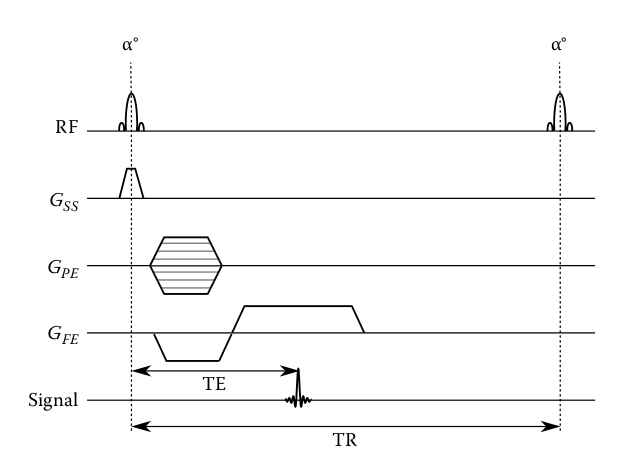
\includegraphics[width=0.7\linewidth]{gre_simplified}
	\caption{Simplified diagram of the GRE sequence that depicts the refocusing gradient applied in the frequency encoding direction \parencite[p.233]{berry_fundamentals_2009}.}
	\label{fig:gresimplified}
\end{figure}

After a series of rf pulses are delivered, we reach a condition in gradient echo sequences called the \textbf{steady state.} In this state, the magnitude of the longitudinal magnetization component $M_z$ is the same at the end of every TR. Similarly, we can also have a residual transverse magnetization $M_{xy}$ at the start of every repetition cycle. If we deliberately dephase this residual transverse magnetization, the sequence is described as incoherent or spoiled gradient echo sequences.

FLASH is a type of spoiled GRE. It is a naming scheme adopted by Siemens that spells Fast Low-Angle Shot. Other vendors have their own naming schemes for such a sequence. General Electric calls it Spoiled Gradient Echo (SPGR) and Philips calls it by the name $T_1$ fast field echo (T1-FFE). \parencite[p.583]{bernstein_handbook_2004}. The introduction of the FLASH technique in the 1980s, known for its rapid acquisition capabilities, marked a significant advancement in MRI technology. It allowed for clearer imaging of dynamic processes and reduced artifacts associated with movement. The original paper on FLASH highlights the technique's potential for 'recording NMR movies' to visualize physiological changes, a capability now fully integrated into contemporary MRI practices." \parencite{haase_flash_1986}

\subsection{Research Necessity}
With the advanced capabilities to capture high-resolution CINE MRI images of the knee during flexion-extension cycles under both loaded and unloaded conditions, we are now faced with the challenge of extracting meaningful biomechanical insights from this data. The first critical step in any such analysis typically involves segmenting the key anatomical structures within the images—namely, the femur and tibia. This process is crucial because accurate segmentation directly influences the reliability of subsequent biomechanical measurements.

Manual segmentation, while simple, is exceedingly time-consuming and susceptible to human error, highlighting the need for more efficient methodologies. In response, this thesis proposes the development of a semi-automated segmentation pipeline. This approach aims to reduce the manual effort required while maintaining high accuracy, thereby accelerating the analysis process and reducing potential biases introduced by manual methods.

Once segmentation is achieved, the next step involves measuring a biomechanical parameter-specifically, the distance between chosen anatomical landmarks on the femur and tibia. This measurement serves as an indirect indicator of joint space, which is crucial for assessing knee health. Derived from 2D images captured in the sagittal plane throughout the knee's flexion-extension cycle, this parameter allows for an analysis of how relative positions between the femur and tibia vary under different conditions of movement and load.

\subsection{Thesis Structure}
Structure of the thesis is as follows: 


\section{Methodology}
\label{sec:second}

\subsection{Data Collection Methods}

\subsubsection{Procedure Details}
Dynamic MRI scans were conducted on four healthy individuals, ranging in age from 28 to 37 years and weighing between 55 to 90 kilograms, utilizing a 3 T Siemens Prisma fit scanner. These volunteers were free from any known musculoskeletal disorders and provided their written consent, adhering to the ethical standards approved by the institutional review board. For all of these subjects, the left leg was scanned. 


Once the subject was placed supine in the scanner, the thigh was secured on a wedge positioner, and the lower leg was attached to an ankle rest, just above the malleoli, using Velcro straps to minimize lateral movement. The knee to be examined is aligned with the device’s axis of rotation, while the other leg rests alongside the MRI scanner's bore.  Knee motion is guided by a belt and sprocket assembly running alongside the lower leg, connected to a gearbox activated by the leg support as the participant flexes and extends the knee. Once the subject was positioned at the scanner's isocenter, their leg naturally assumed a flexed posture due to the design of the device. In this configuration, the leg is cradled by the device arm which is positioned below the level of the knee, ensuring that the leg remains flexed without the volunteer exerting any force.


The volunteer engaged in a controlled exercise, following a metronome set at 60 beats per minute. This pace dictates a four-beat flexion to extension cycle, with the leg being flexed at the first beat and fully extended by the fourth. This equals to 8 beats per cycle, or 7.5 cycles every minute. Initially conducted under a loaded condition with weights added to the distal end of the device, the process is repeated without the added resistance to compare both states. The scan duration is around two and a half minutes, amounting to 20 full flexion-extension-flexion cycles. 

\subsubsection{Sequence Parameters and Reconstruction}
Table \ref{tab:mri_seq_params}, lists the MRI sequence parameters along with their respective units.

\begin{table}[H]
	\centering
	\label{tab:mri_seq_params}
	\caption{MRI Sequence Parameters}
	\begin{tabular}{@{}ll@{}}
		\toprule
		Sequence Parameters & Values \\ \midrule
		Shape & (352, 276, 16, 100) \\
		Acquisition Duration & 160 [s] \\
		Acquisition Type & 2D \\
		Dwell Time & 0.0024 [s] \\
		Echo Time & 2.51 [ms] \\
		Field Strength & 2.89362 [T] \\
		Flip Angle & 8.0 [degrees] \\
		Field of View (FOV) & 192.0 x 192.0 x 3.0 [mm] \\
		Frequency & 123.25 [MHz] \\
		Inversion Time & 150000 [ms] \\
		Matrix Size & 176 x 176 x 1 \\
		Repetition Time & 5.8 [ms] \\
		Scanner Name & MAGNETOM Prisma \\
		\bottomrule
	\end{tabular}
\end{table}

In this study, the k-space data was acquired using 16 receive channels, each recording data simultaneously but with a unique spatial sensitivity profile. With 276 spokes used to sample a k-space dataset and a repetition time (TR) of 5.8 milliseconds per spoke, it takes approximately 1.6 seconds to acquire one k-space data. Over the course of the experiment, 100 such k-space datasets are acquired, equaling 100 repetitions as noted. The total scan duration extends just over two and a half minutes, a time frame reported by the subjects as being manageable, regardless of whether the scan was conducted under loaded or unloaded conditions.

Each k-space dataset contained data across a range of knee angles because of the continuous leg movement set to the metronome beat. This means, assuming the subjects perform perfectly in time of 60 beats per minute where we have 4 beats for flexion to extension, each k-space covers 0.4 times the range of motion. For example, a subject with a range of motion of $40^o$, each k-space dataset contains data across $16^o$. Therefore, with multiple repetitions, data across the full range of motion could be adequately acquired.     
 

To illustrate the principle of radial k-space sampling, Figure X presents a simplified model, which includes only a few spokes and sampling points for visual purposes. In practice, as given in table \ref{tab:mri_seq_params}, we have 352 points per spoke, and 276 spokes in total per k-space. 

\begin{figure}[H]
	\centering
	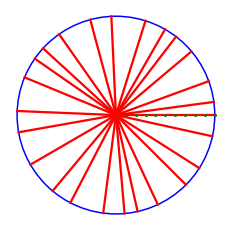
\includegraphics[width=0.7\linewidth]{kspace_depiction}
	\caption{This illustration depicts a radial sampling pattern with 25 red spokes, using the golden angle for spacing. Only one spoke is detailed, showing 10 green points to represent sampling positions.}
	\label{fig:kspacedepiction}
\end{figure}

\textbf{Reconstruction}


The MRI raw data, with dimensions of (352, 276, 16, 100), was processed using a reconstruction script to generate the final image dataset. First, the binary data from the optical sensor was loaded, and the physical angle information was grouped according to each repetition cycle. This was done by detecting significant changes in the trigger signal, which was obtained from the sensor data too. This grouping resulted in 100 groups, each containing the physical angle information for a specific repetition. For each repetition, spokes in k-space were assigned to their corresponding physical angles. An angle increment of 2 degrees was chosen, which led to a collection of spokes corresponding to each 2-degree range. This approach was applied to all repetitions, allowing spokes to be mapped to physical angles across the full range of motion.

Subsequently, reconstruction was performed on each group of spokes. Depending on the specific angle range, the number of spokes assigned varied between 300 and 1000. Additionally, the direction of leg movement—either from flexion to extension or vice versa—was determined by calculating the slope of the angle information. Images were then reconstructed separately for each direction, depending on whether the leg was moving upward or downward. This distinction is crucial because leg biomechanics vary significantly depending on whether the movement is working with or against gravity.

\textbf{The use of rielsing toolbox}

The actual image reconstruction was done by using the Riesling reconstruction toolbox \parencite{wood2020riesling}. This toolbox offers a range of advanced algorithms tailored for non-Cartesian MRI reconstruction. In this study, an Alternating Direction Method of Multipliers (ADMM) approach was employed, incorporating Total Generalized Variation (TGV) regularization. 

ADMM is an iterative optimization algorithm that breaks down complex problems into smaller subproblems to solve them efficiently. It ensures accurate reconstruction by maintaining a balance between the primal (actual solution) and dual (approximate solution) residuals. This balance is particularly important for non-Cartesian MRI reconstruction, given the unique geometry of the data. ADMM allows different regularization techniques, like TGV, to be applied simultaneously during reconstruction.\parencite{MAL-016} 

TGV is an advanced regularization method that reduces noise while promoting smoothness in the reconstructed images. Unlike basic Total Variation (TV) regularization, TGV allows for piecewise smooth transitions between different regions, making it better suited for images with varied structures. In this study, a regularization strength of 5e-2 was chosen empirically, striking a balance between noise suppression and edge detection.

The final reconstructed images were affected by the chosen reconstruction parameters, including the zero-filling factor and the field of view (FoV) trimming factor. The use of TGV regularization and the ADMM algorithm influenced the resulting image resolution, providing images with a consistent size suitable for downstream analysis. Each image frame was reconstructed with dimensions of (528, 528) and the number of frames were subject dependent. 


\subsection{Data Analysis}
All the analysis and data visualization were done using the python programming language (v3.11.5). To begin, the data in nifti (Neuroimaging Informatics Technology Initiative) format is loaded using nibabel (v5.1.0) library. It is then visualized using napari(v0.4.18), a multi-dimensional interactive image viewer in Python. Figure \ref{fig:step1viewer} shows the initially loaded data along with the viewer user interface. 
\begin{figure}[H]
	\centering
	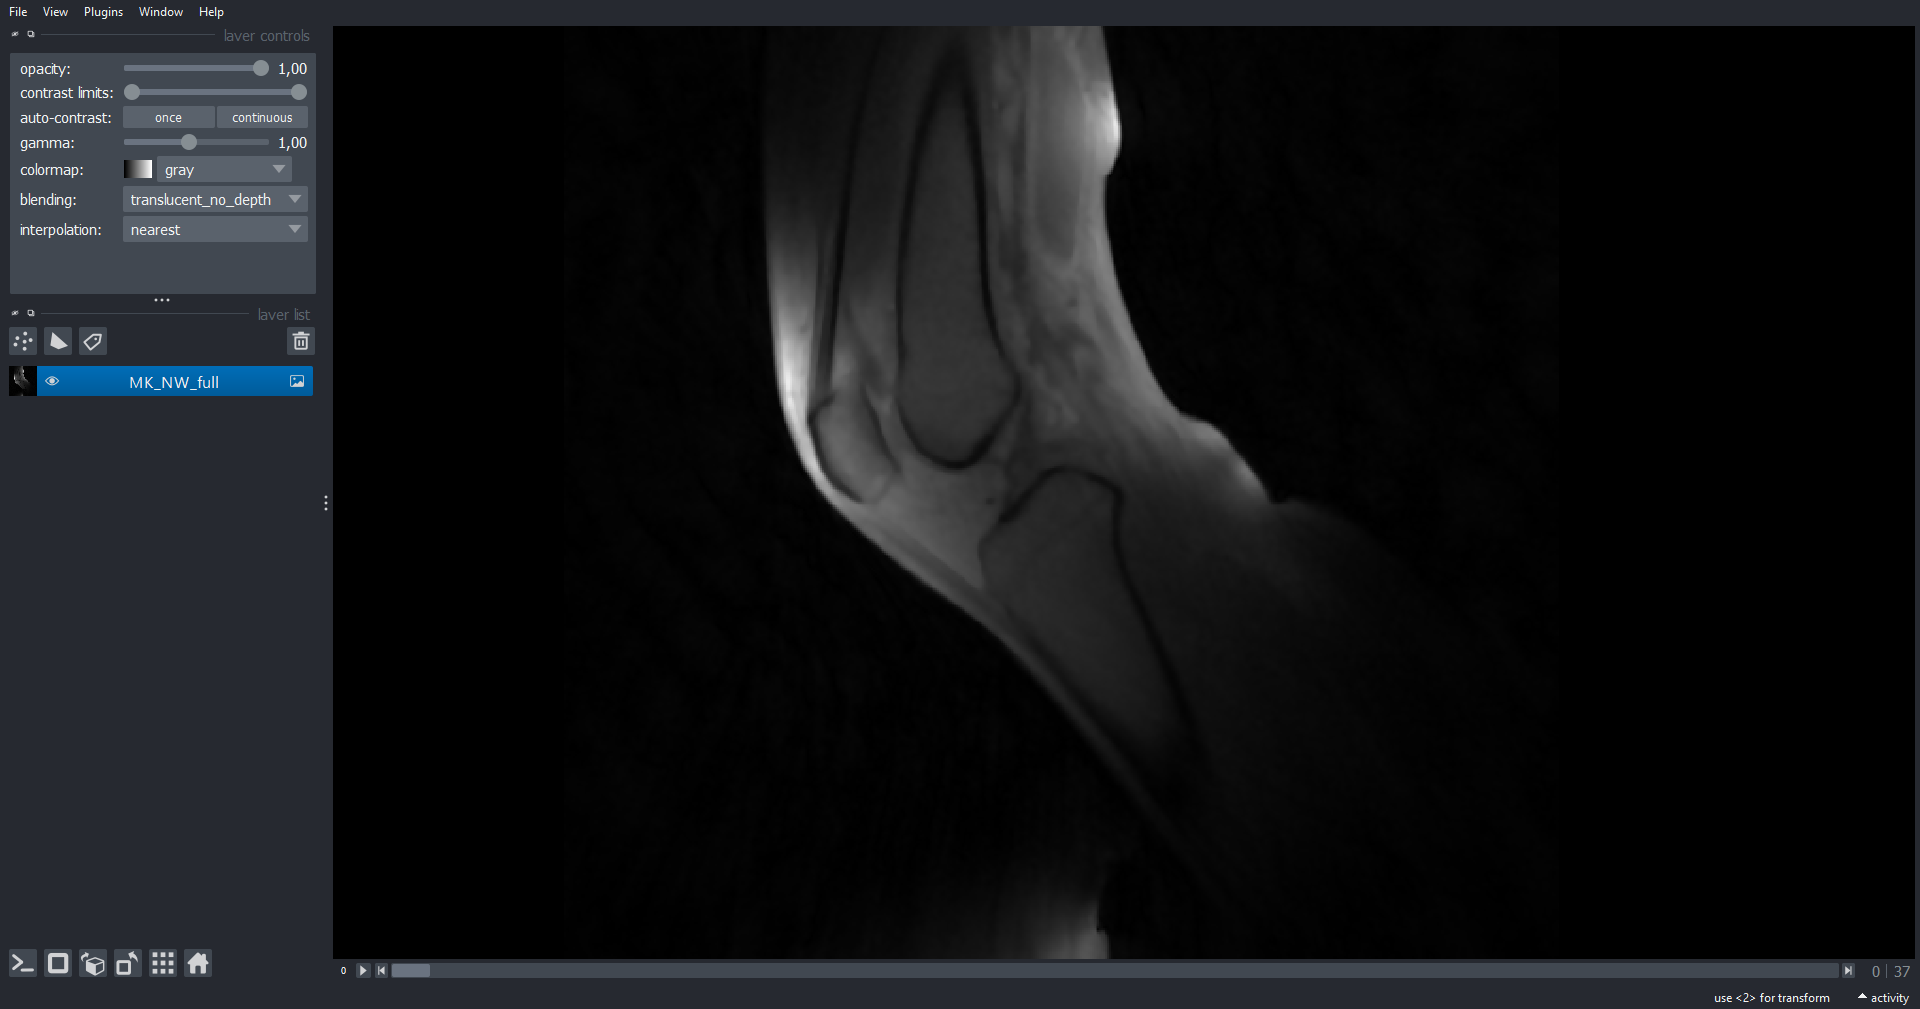
\includegraphics[width=0.7\linewidth]{step_1_viewer}
	\caption{An example of the layout of the Napari viewer application showing one of the frames of CINE data.}
	\label{fig:step1viewer}
\end{figure}

Once the data is loaded, several distinct steps were performed to semi-automate the segmentation of tibia and femur. This involves first finding one boundary edge each for the bones, and then tracking them across the full flexion-extension cycle by computing their respective transformation matrices. 
 
\subsubsection{Segmentation}
\textbf{Step 1: Edge Detection}

The Canny filter \parencite{canny_computational_1986}, as implemented in the scikit-image's feature library (v0.21.0), was employed to apply an edge filter to the images. The Canny edge detection algorithm operates in several key steps to identify edges with high accuracy in images. Initially, the image is smoothed using a Gaussian filter to reduce noise and potential false edge detections. Following this, the algorithm calculates the gradient intensity and direction at each pixel, which helps in identifying the edges' boundaries.

Subsequently, the algorithm applies double thresholding, which involves two thresholds: a low and a high. Pixels with intensities above the high threshold are marked as strong edge pixels, while those below the low threshold are discarded. Pixels between these two thresholds are marked as weak edge pixels but can only be accepted as true edge pixels if they are connected to strong edge pixels. This step helps in discriminating between real edges and noise. Finally, edge tracking by hysteresis completes the process by converting weak edge pixels that are connected to strong edge pixels into strong edges, ensuring the continuity and completeness of detected edges in the image. Various parameters of the Canny algorithm were adjusted, including edge thresholds and Gaussian blur, to optimize edge detection. Figure \ref{fig:edgemitimg} shows the output of this step.  
\begin{figure}[H]
	\centering
	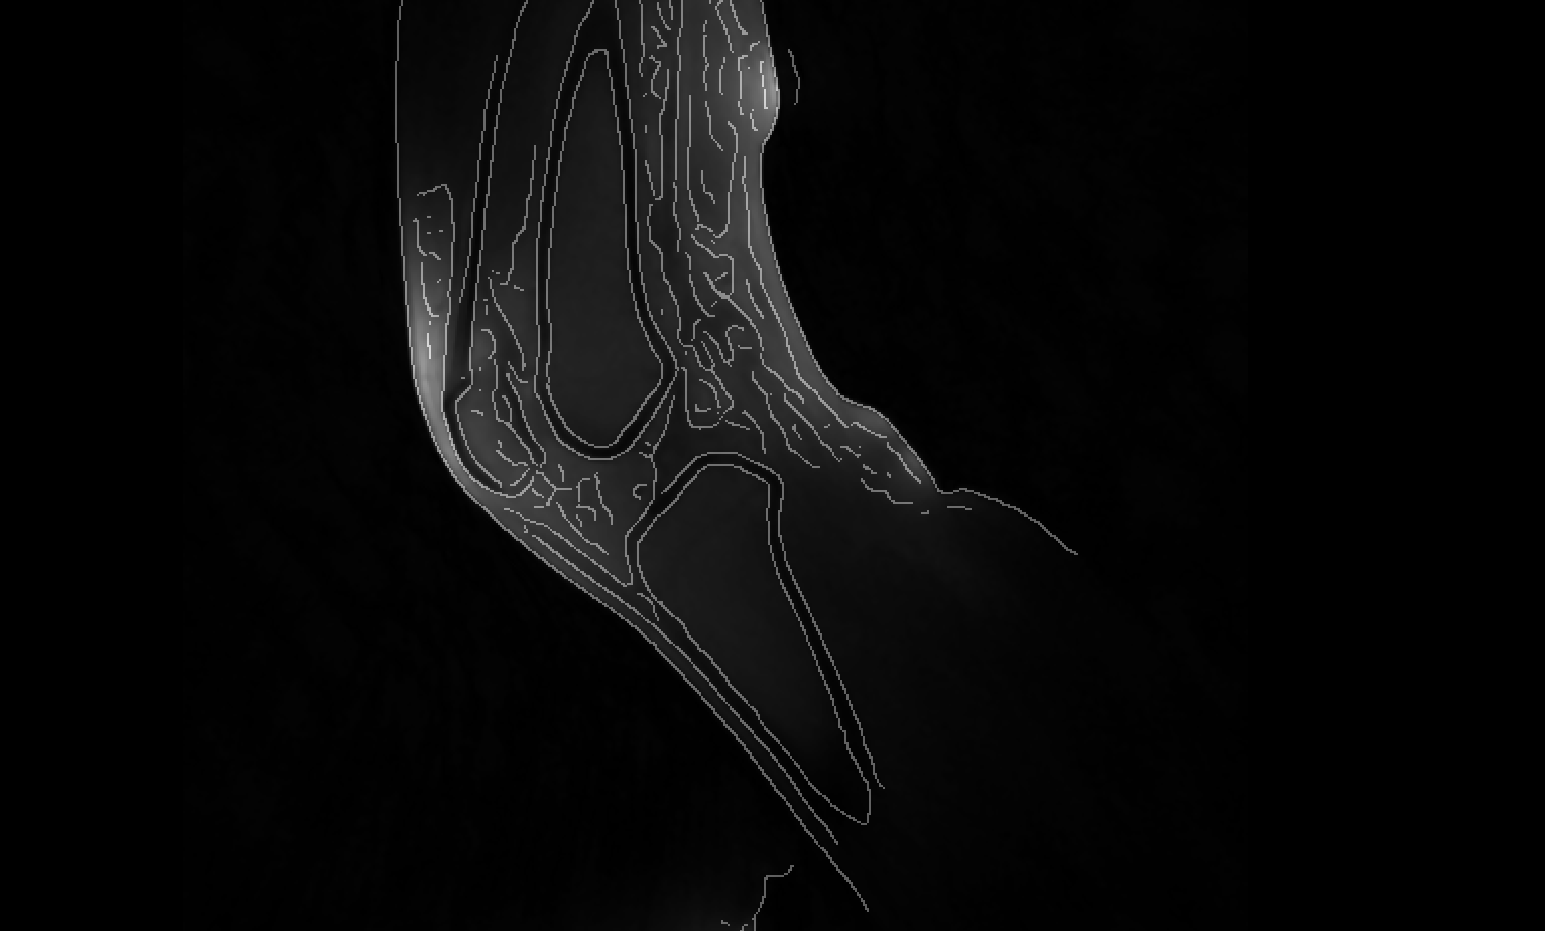
\includegraphics[width=0.7\linewidth]{edge_new}
	\caption{Output of canny edge detection algorithm overlayed on top of the image.}
	\label{fig:edgemitimg}
\end{figure}


Subsequently, the scikit-image's morphology library was utilized to remove small elements from the binary image. The image was then skeletonized to a one-pixel width, retaining only long and consistent edges. It should be pointed out that the final edge does not necesarrily need to span the full boundary of the interior edge of the cortical bone; even partial edges were successfully used for this purpose.  

\textbf{Step 2: Labelling}

For the final selection of the desired edge, a labeling algorithm from SciPy, an open-source Python library designed for scientific computing(v1.11.3) was used. The goal was to isolate an edge that accurately represents the overall shape of the bone slice. Labelling was useful in this regard as it allowed for easy separation of distinct edges. Figure \ref{fig:labelimg} shows the output from the labelling algorithm, where each color represents a separate label. 

\begin{figure}[H]
	\centering
	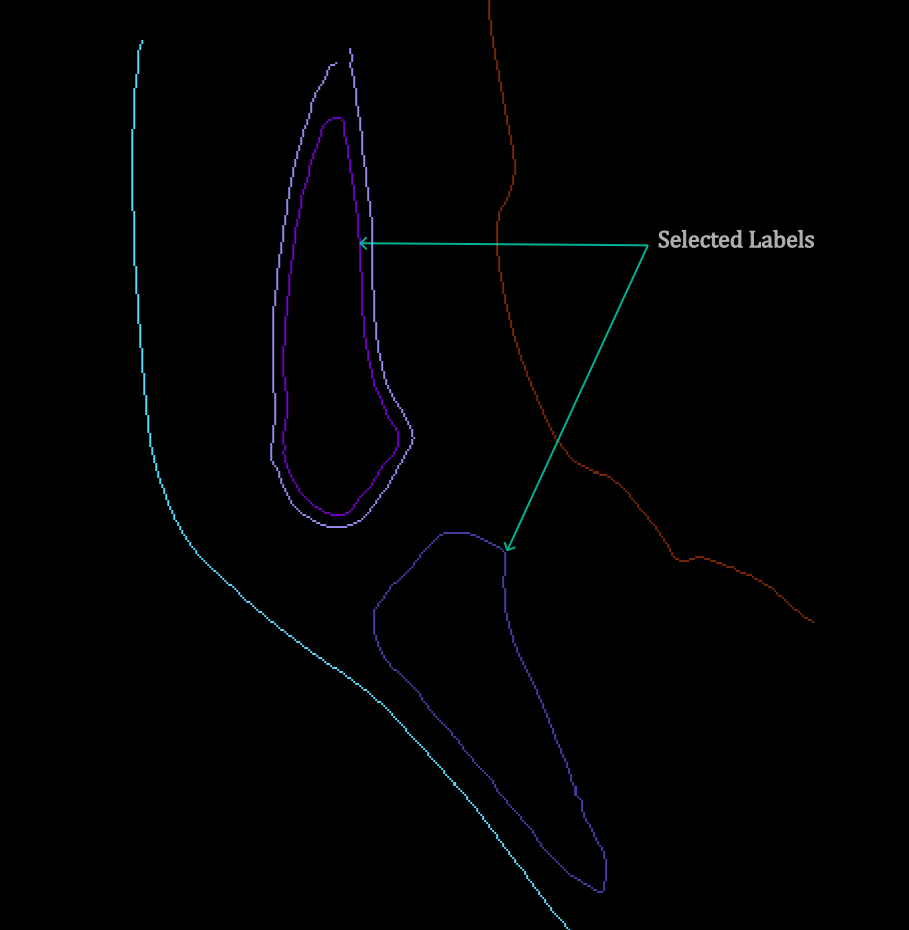
\includegraphics[width=0.7\linewidth]{label_selected}
	\caption{Output from the labeling algorithm with the representative edges for femur (top) and tibia(bottom) pointed out.}
	\label{fig:labelimg}
\end{figure}
 
After choosing the appropriate labels, a binary image for each frame is obtained, where the foreground has the boundary for the interior edge of tibia and femur, and the background is null.   

\textbf{Step 3: Obtaining the set of reference points}

Upon successfully isolating the binary edge images of the tibia and femur in Step 2, the subsequent step deals with establishing a set of reference points along each bone's edge in the first frame. This frame, captured when the knee is in a fully flexed position, serves as the reference frame for the study. The purpose of establishing these reference points is twofold: to simplify the complex data set for efficient processing and to ensure a consistent basis for accurately calculating transformations between subsequent frames. This is essential, as direct use of the densely packed binary edge data would be computationally cumbersome and less precise for such transformations.

To begin, the points along the boundary were organised and sorted. This was done by first, defining a starting point, and then iteratively using a greedy nearest neighbor algorithm for sorting. The most distal point of the bone was taken as the initial seed. Various functions from the numeric python library 'Numpy' (v. 1.26.4) were employed for this task. 


Once the points are sorted, the next step involves downsampling these points to a set of uniform equidistant reference points along the boundary of the binary edge. The necessity for this step arises from the inherent irregularity and density of the binary edge data. Directly sampling every nth point from the sorted list would not suffice, as it could result in uneven spacing due to the variable distances between consecutive points in the original data.

This process begins by calculating the cumulative distances between each consecutive pair of points in the sorted list. Using these distances, a total path length is established. The desired interval between the new points is then determined by dividing this total path length by the number of intervals (number of desired points minus one). Between 50 to 80 points were found to be sufficient to accurately reflect the edge contours. 

To achieve precise positioning of these points, cubic spline interpolation from SciPy's interpolate libary is used. This interpolation method is particularly effective for ensuring that the new points adhere closely to the original curve while maintaining equidistant. 
Figure \ref{fig:downsampled} depicts this result. 
\begin{figure}[H]
	\centering
	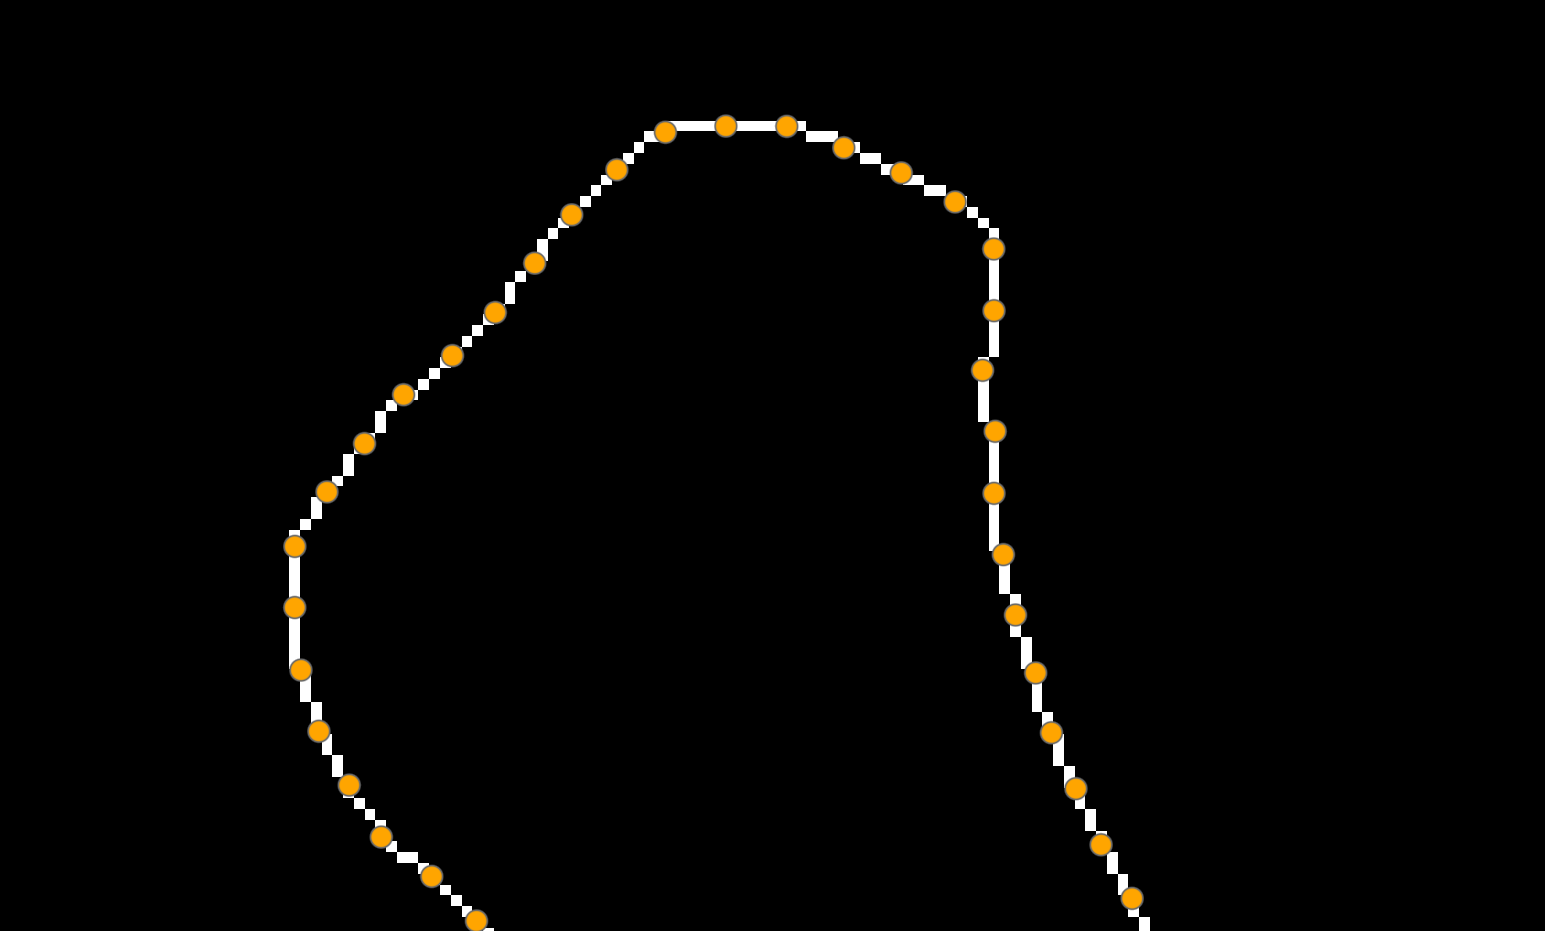
\includegraphics[width=0.7\linewidth]{downsampled}
	\caption{A zoomed in look at the equidistant sampled points (orange) along the boundary of the tibia edge (white).}
	\label{fig:downsampled}
\end{figure}

\textbf{Step 4: Transformation matrices computation}

In this step, a set of transformation matrices are obtained, each matrix containing the paramters that align the segment of the bone in one frame to the next. Given that the subject movement is restricted to only a single plane, it is reasonable to assume that the edges of the bone undergo motions that can be described by rigid transformations. These transformations includes solely the translation in the sagital plane, and rotation about transverse axis. In this approach, it is assumed that the bone does not undergo any deformation, and that through plane motion is negligible throughout the motion cycle. 

Mathematically, the transformation of each point from one frame to the next can be expressed as 
\begin{equation}
	p^{'} = R(\phi)p + t
	\label{eq:rot} 
\end{equation}
where: 
\begin{itemize}
	\item \textbf{$p$} is the coordinate of the point in its current frame
	\item \textbf{$p^{'}$} is the coordinate of the point in the next frame
	\item $\phi$ is the angle of rotation
	\item \textbf{$R(\phi)$}  is the rotation matrix, given by 
	 \[
	 R(\phi) = 
	 \begin{bmatrix}
	 	\cos \phi & \sin \phi \\
	 	-\sin \phi & \cos \phi
	 \end{bmatrix}
	 \]
	 \begin{itemize}
	 	\item $t$ is the translation vector,
	 	\[
	 	t = \begin{bmatrix}
	 		x \\
	 		y
	 	\end{bmatrix}
	 	\]
	 \end{itemize}
 	\item x and y are the translations in the cartesian coodinate system. 
\end{itemize}   
As such, only three parameters, $x$, $y$, and $\phi$ need to be computed. To compute these, a cost function is defined that measures the sum of squared distances between each point in the reference frame and its corresponding point in the transformed frame. The optimization of this cost function is performed using a nonlinear least squares approach, where the initial guess is provided. The optimization process uses the fmin function from SciPy’s optimization module, which is configured to stop when the change in the cost function is below a small tolerance, ensuring precise alignment of the frames. This method ensures that the computed transformations accurately represent the actual movements of the bone throughout its movement cycle. Figure \ref{fig:edge_tracking} provides a visual representation of the overlap of the reference points from the fully flexed initial position to the frame where the lower leg has been rotated by an angle of 12 degrees as reported by the rotary angle encoder. 
\begin{figure}[H]
	\centering
	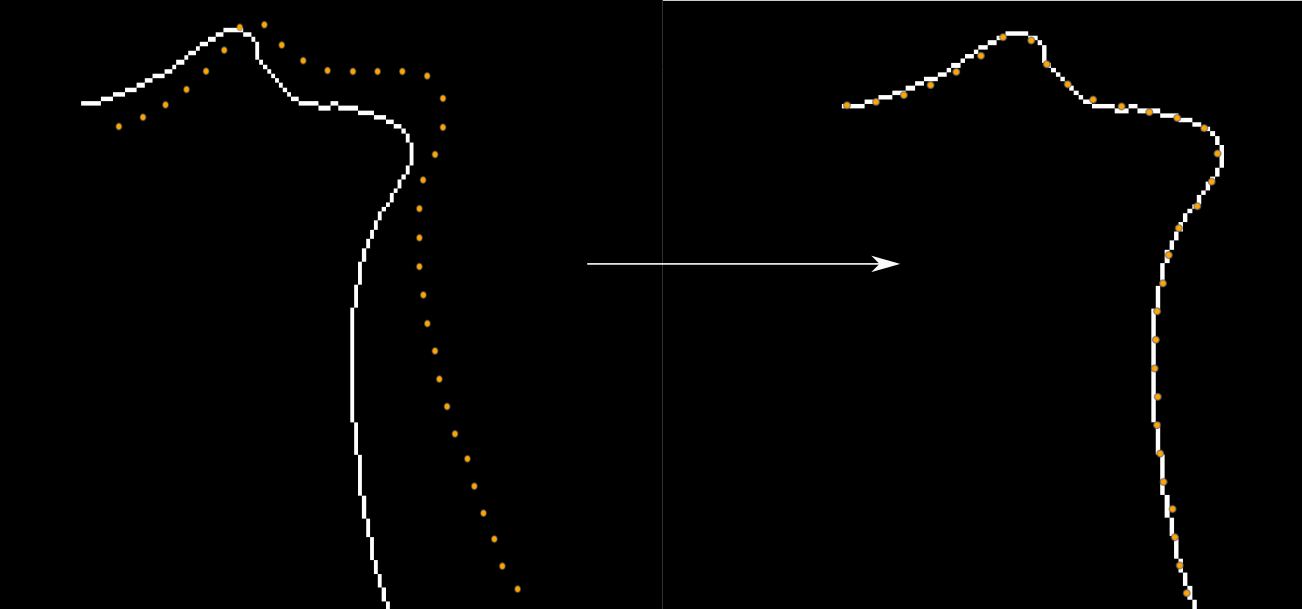
\includegraphics[width=0.7\linewidth]{image137}
	\caption{Left: The reference points in the first frame (orange) overlayed with the binary edge image of the target frame (white).Right: The reference points have been transformed by using the results from the optimization showing almost perfect overlap, illustrating the effective alignment achieved through the minimization of the cost function.}
	\label{fig:edge_tracking}
\end{figure}

\textbf{Step 5: Auto-Segmentation }

With the transformation matrices obtained for the femur and the tibia, manual segmentation is performed on the first frame. An example is given in figure \ref{fig:manualsegment}. 
\begin{figure} [H]
	\centering
	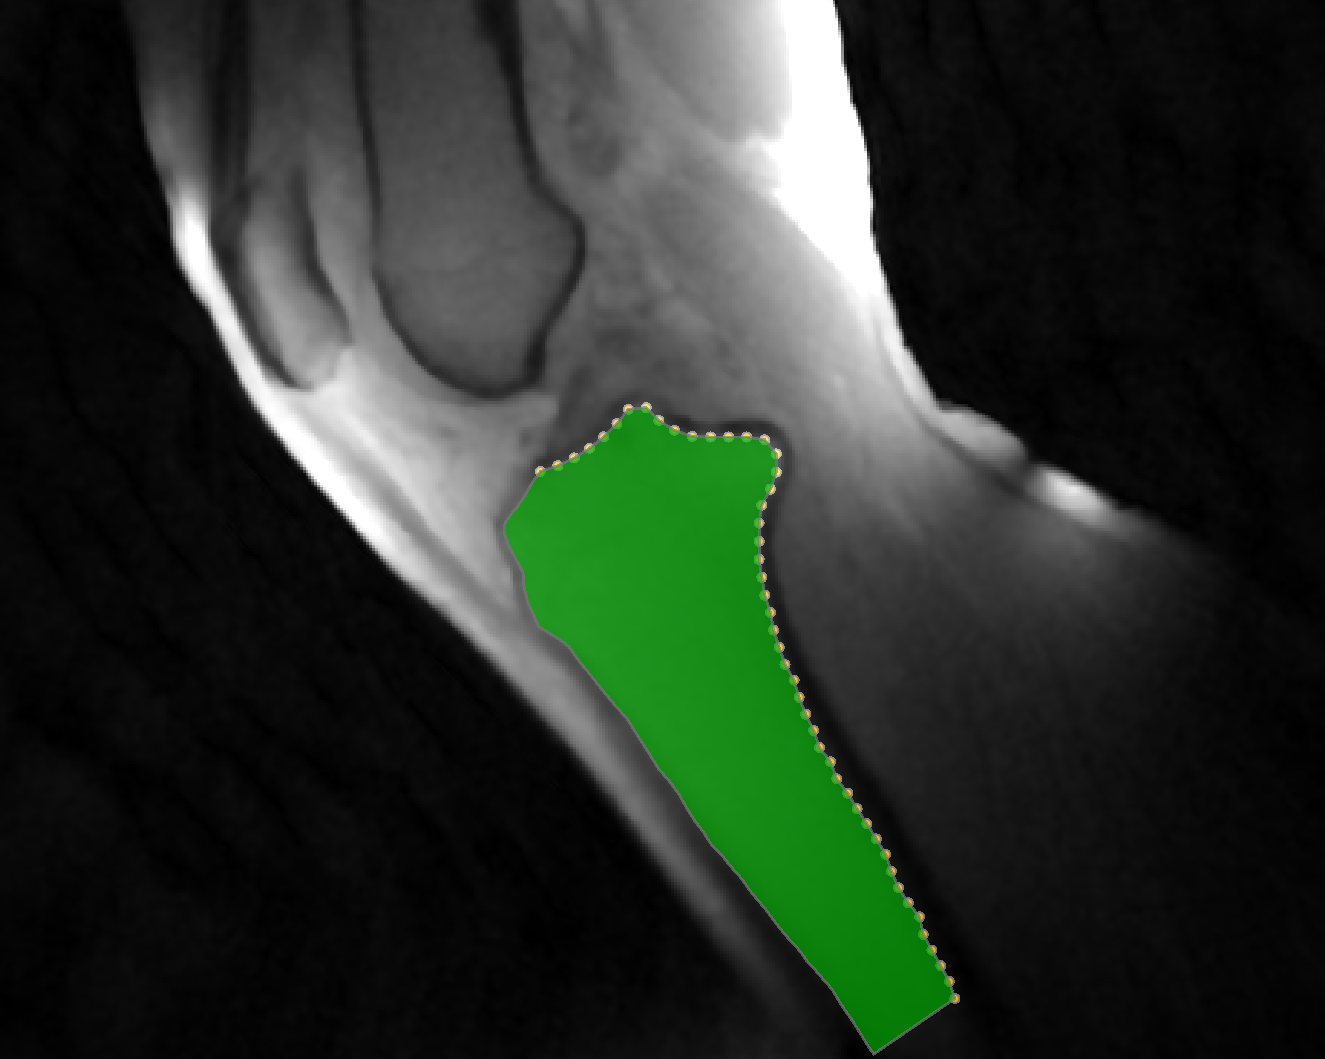
\includegraphics[width=0.7\linewidth]{manual_segment}
	\caption{Manual segmentation is performed to complete the boundary of the tibia's interior edge shown in green, along with the reference points (orange).}
	\label{fig:manualsegment}
\end{figure}

Using the points from this segment, the transformation matrices are now applied once more using equation \ref{eq:rot} to transform one frame to the next subsequently to complete the full segmentation across all the frames automatically. The result of the segmentation for one of the datasets is given in figure blank. 

\begin{figure}[H]
	\centering
	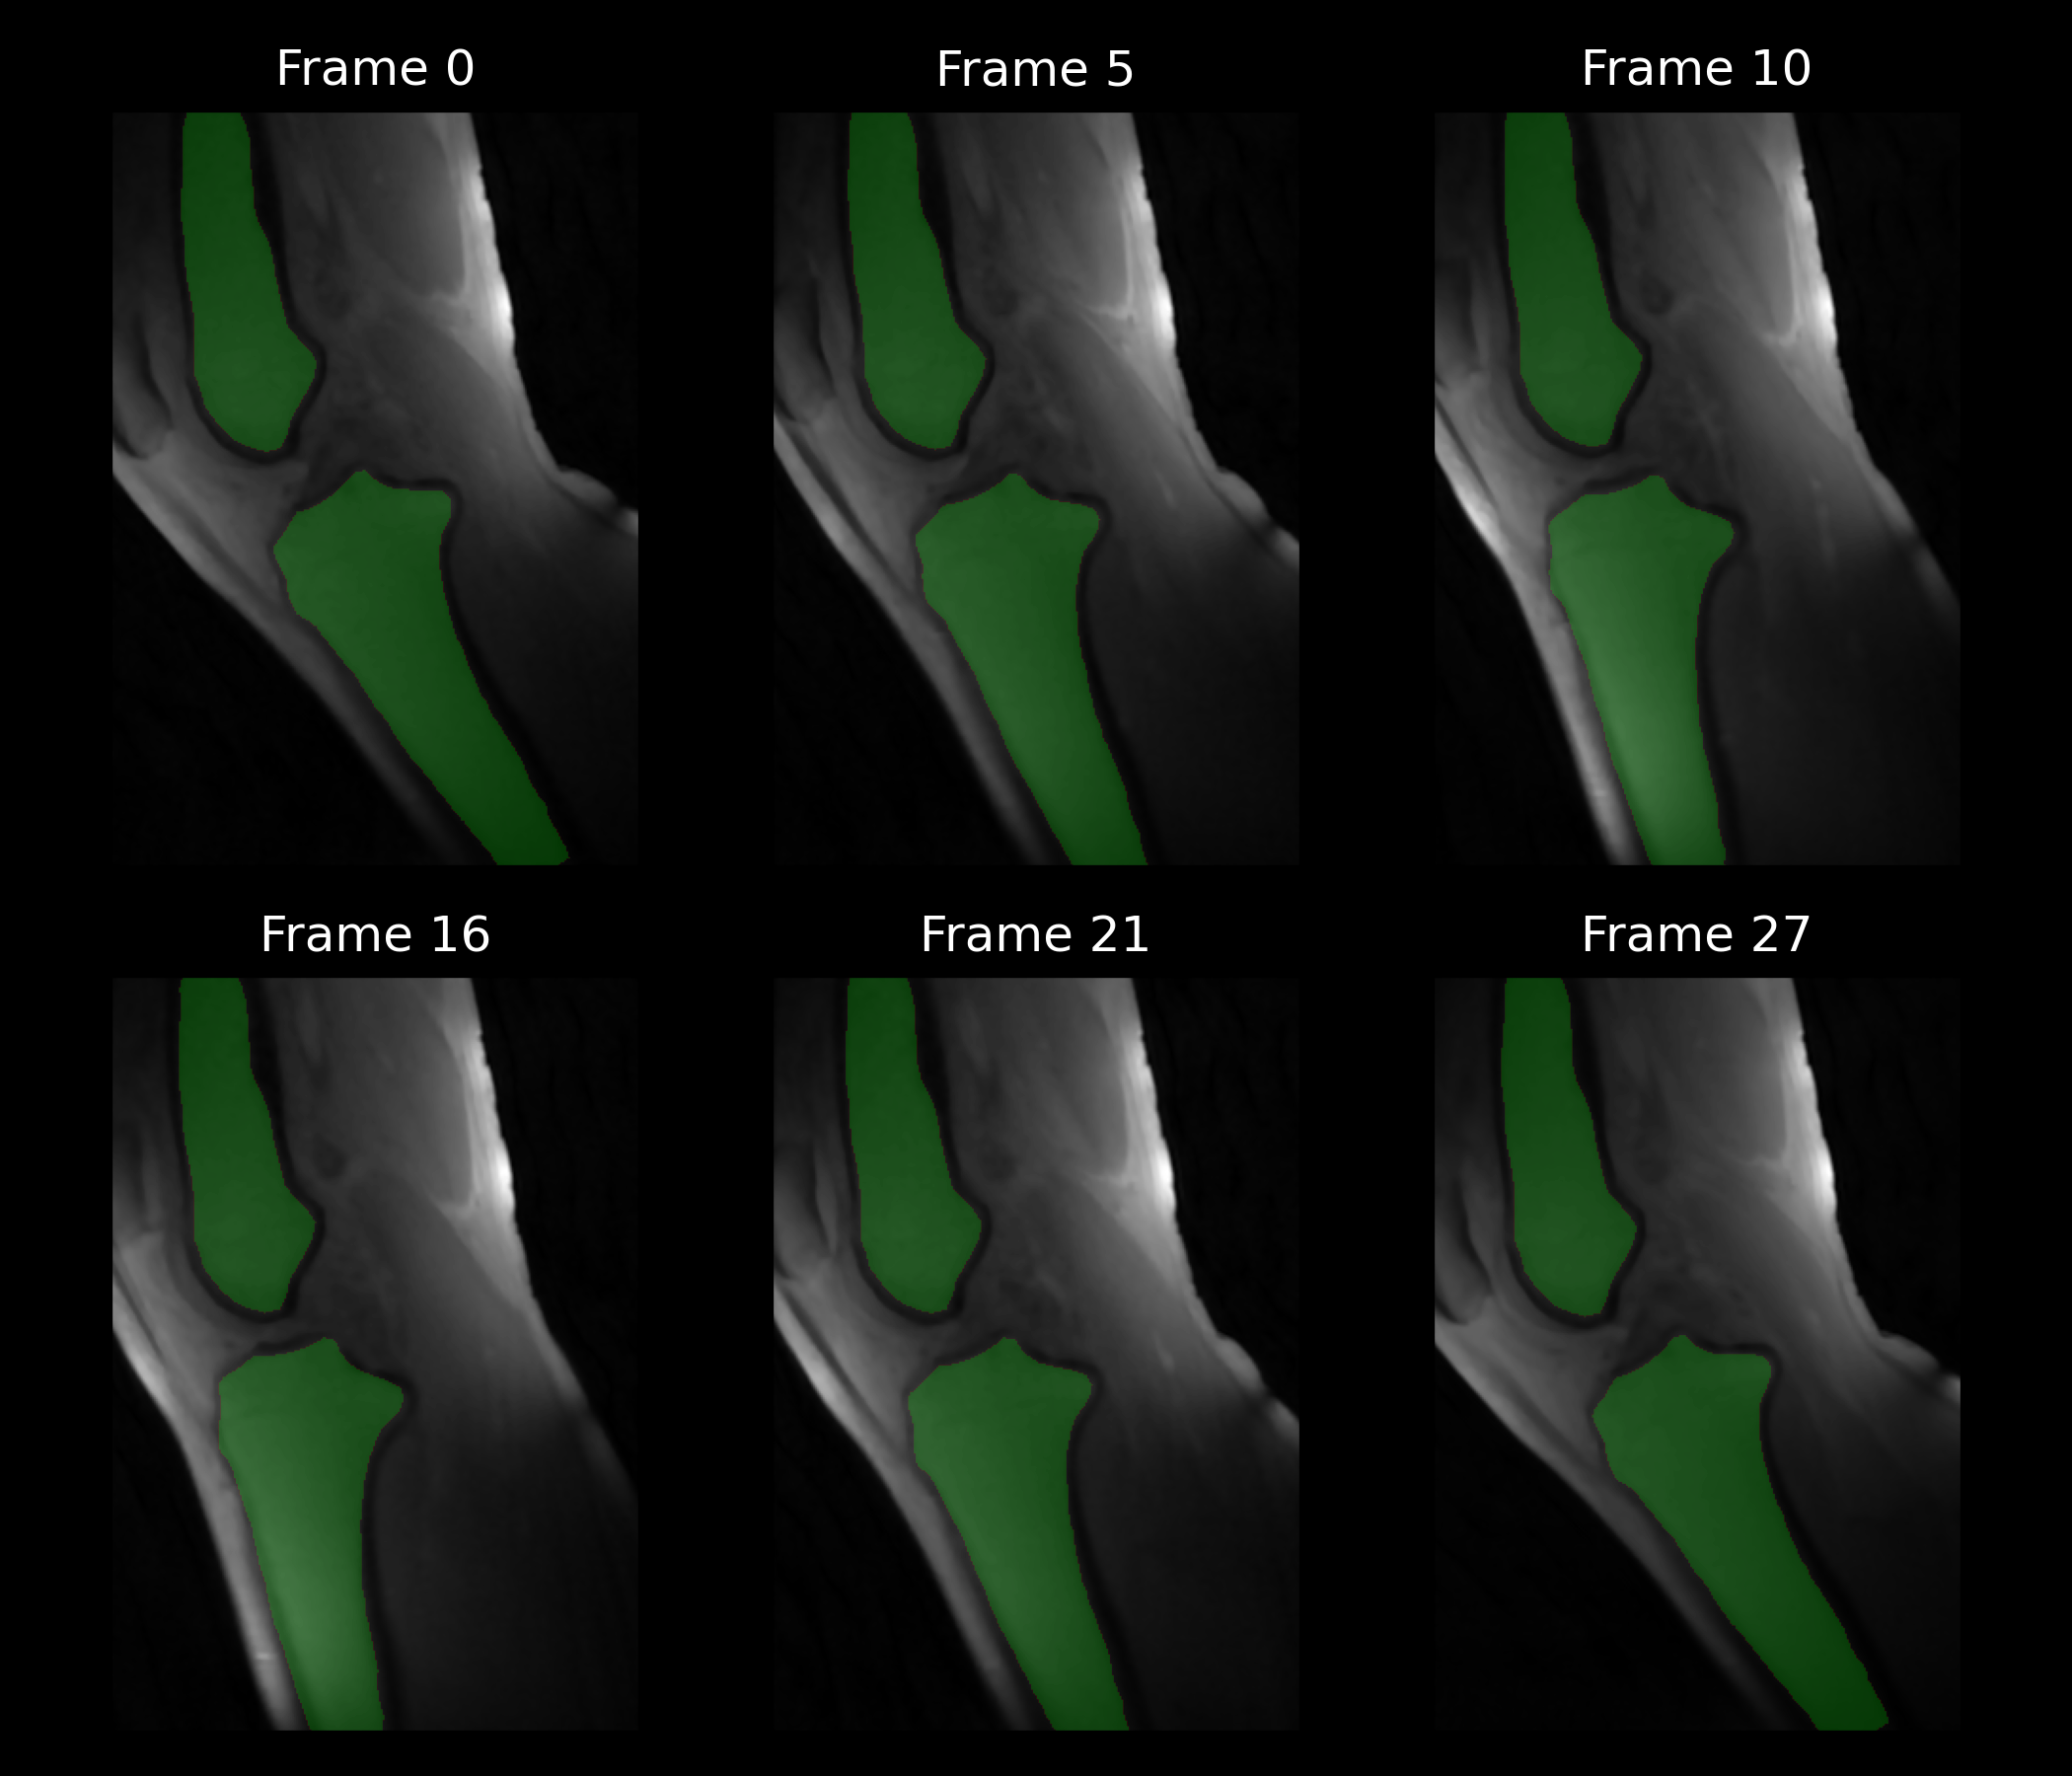
\includegraphics[width=0.7\linewidth]{full_segmented}
	\caption{A mosaic showing the segmented tibia and femur shapes(green) where each tile is a particular time point. The leg is fully flexed at Frame 0}
	\label{fig:fullsegmented}
\end{figure}
  

\subsubsection{Extraction of Biomechanical Parameters}
After achieving automated segmentation of the tibia and femur across all frames, the next step involved extracting biomechanical parameters from the segmented regions. Two key metrics were considered for analysis to assess the relationship between these bones throughout the flexion-extension cycle captured in the 2D Cine images.

The first metric involved calculating the angle between the long axis of femur and tibia segments. This measurement provided insight into how the relative orientation of the two bones changes over time.

The second metric measured the distance between specific anatomical landmarks on both the femur and tibia. Tracking this distance across the frames offered an understanding of how the spatial relationship between these two bones evolved during the motion cycle. 

\textbf{Angle between the bones}

To calculate the angle between the bones, the long axis of each bone segment was identified using a technique called Principal Component Analysis (PCA). The analysis was performed using the PCA implementation from the scikit-learn (v1.3.1) Python library, a module for machine learning built on top of SciPy.

PCA determines the direction of maximum variance in the data, which coincides with the long axis of the bone. PCA first uses the coordinates of the segmented binary mask as input. The centroid of the shape is calculated and subtracted from each data point, centering the data such that the mean of this transformed data is (0, 0). 

Next, the covariance matrix (\text{Cov}) is computed, a square matrix that gives an indication of how the data varies along each dimension and how different dimensions vary together. 

\begin{equation}
	\text{Cov} = 
	\begin{bmatrix}
		\mathrm{Var}(X) & \mathrm{Cov}(X,Y) \\
		\mathrm{Cov}(Y,X) & \mathrm{Var}(Y) \\
	\end{bmatrix}
	\label{eq:cov}
\end{equation}

where:
\begin{itemize}
	\item \(\mathrm{Var}(X)\) is the variance of \(X\), given by:
	\[
	\mathrm{Var}(X) = \frac{1}{N-1} \sum_{k=1}^{N} (X_{k} - \bar{X})^2,
	\]
	where \(N\) is the number of points, \(X_{k}\) represents the \(k^{th}\) observation in the \(X\) dimension, and \(\bar{X}\) is the mean value of all observations in the \(X\) dimension. 
	\item \(\mathrm{Cov}(X,Y)\) is the covariance between dimensions \(X\) and \(Y\), defined as:
	\[
	\mathrm{Cov}(X,Y) = \frac{1}{N-1} \sum_{k=1}^{N} (X_{k} - \bar{X})(Y_{k} - \bar{Y}),
	\]
	where \(Y_{k}\) represents the \(k^{th}\) observation in the \(Y\) dimension, and \(\bar{Y}\) is the mean value of all observations in the \(Y\) dimension.
	
	\item \(\mathrm{Cov}(Y,X)\) is equivalent to \(\mathrm{Cov}(X,Y)\) because the covariance matrix is symmetric.
	
	\item \(\mathrm{Var}(Y)\) is the variance of \(Y\), calculated similarly to \(\mathrm{Var}(X)\).
\end{itemize}

Once we have the covariance matrix, we compute its eigenvectors and eigenvalues. The eigenvector corresponding to the largest eigenvalue points in the direction of maximum variance, which is the first principal component. In this specific case, the first principal component aligns with the long axis of the tibia segment.


\textbf{Distance between the bones}
This is how the distance between the bones are calculated. 


\section{Results}
\label{sec:yetanother}



\section{Discussion}

 

\section{Conclusion}


% ----------------------------------------------------------------------------
% Bibliography
% ----------------------------------------------------------------------------
\cleardoublepage
\phantomsection
\addcontentsline{toc}{section}{\refname} % to add Bibliography to toc
\printbibliography

% --------------------------
\cleardoublepage
\begin{appendix}
\section{Appendix}
If needed for supplementary material, such as detailed description of data collection, tables, or figures.

\end{appendix}

% ----------------------------------------------------------------------------
% Statutory declaration
% ----------------------------------------------------------------------------
\makeThesisDeclaration

\end{document}

